\documentclass[onecolumn, a4paper, oneside, article, 12pt]{report}
\usepackage[utf8]{inputenc}
\usepackage{graphicx}
\usepackage{float}
\usepackage[hidelinks]{hyperref}
\usepackage{listings}
\usepackage{isotope}
\usepackage{color}
\usepackage{mathtools}
\usepackage{amsmath}
\usepackage{siunitx}
\usepackage{amssymb} % extra math symbols
\usepackage{hyperref}
\usepackage[labelfont=bf]{caption}
\usepackage[table,xcdraw]{xcolor}
\usepackage{wrapfig}
\usepackage{enumitem}
\usepackage{amsmath}
\usepackage{mathtools}
\DeclarePairedDelimiter{\abs}{\lvert}{\rvert}
\usepackage{titlesec}

\titleformat{\chapter}[block]
{\normalfont\huge\bfseries}{\thechapter}{20pt}{}
\titlespacing*{\chapter}
{0pt}{20pt}{20pt}

\setcounter{tocdepth}{5}
\setcounter{secnumdepth}{5}

\hypersetup{colorlinks=true, linkcolor=blue, urlcolor=blue, citecolor=blue}
\setlength{\parindent}{0pt}
\newcommand{\note}{\textcolor{red}}

\DeclarePairedDelimiter{\p}{(}{)}
\DeclarePairedDelimiter{\kp}{[}{]}
\DeclarePairedDelimiter{\set}{\{}{\}}

\makeatletter
%\renewcommand{\@seccntformat}[1]{}
\makeatother


\title{SPECIALE TITEL HER!}
\author{Anders Holst Rasmussen}
\begin{document}
	\maketitle
	
	\chapter{Introduction}
%\begin{enumerate}
%	\item We are interested in the decay, and want to describe what is happening.
%	\item Different levels which gives a continuum of 2+ state.
%	\item \isotope[8]{Li} har spin +2
%	\item We expect 2+ structure in \isotope[8]{Be}
%	\item There exists earlier measurements of \isotope[8]B	made in the AU group.
%	\item \isotope[8]B is the mirror core?? And has been measured very precisely.
%	\item Measure Li with same precision.
%	\item A beautiful spectrum from the alphas.
%	\item Look at a single alpha.
%	\item Look at coincidence.
%	\item Better to look at both and add, recoil will give widening.
%	\item read bataratjaa
%	\item We are interrested in beta alfa angles for \isotope[12]B
%	\item People have measured this angle precisely, because they where looking for deviations in the standard model.
%\end{enumerate}
%
%
%We want to examine the \be-delayed decay of \isotope[8]Li, which is an unstable isotope of Lithium. Lithium normally occurs stable as \isotope[6]Li and \isotope[7]Li, with the latter being the more abundant with 92.5\% of all atoms. The longest living radioactive lithium isotope is \isotope[8]Li, with a half-life of \SI{839}{ms} \note{ref}. 
%
%\li is an interesting atom, as it will decay into \isotope[8]Be, which is a constituent in the triple-alpha process in stellar astrophysics. \isotope[8]Be creates a bottleneck for the creation of heavier elements, as it is very short lived, and have a half-life of \SI{1e-16}{s}.
%
%\li will also decay into \ber at different energy levels, which will give a continuum of the 2+ state from \li. 
%
%The Sub-atomic group at Aarhus University has previously measured decay of the mirror nuclei, \isotope[8]B. Since there exists very precise measurement, we want to ¨obtain similar precise measurements of \li. 

\section{Motivation}
When Henri Becquerel first discovered radioactivity in the 1890's, a new branch of atomic physics was born, namely nuclear physics, which is the study of the atomic nuclei, their constituents and interactions. 
Over the years it has evolved quickly, first by the discovery of three different types of radiation by Curie and Rutherford, to the discovery of different nucleons, that the nucleus itself is made of. \note{måske ref til Curie and Rutherford?} \\
\\
The technological advancements has made the study even more precise over the years, as the development of radioactive beams allow for the creation of specific short lived isotopes.
This technique is known as Isotope Separation On-Line (ISOL), which was first developed in 1951 for the Copenhagen Cyclotron. 
Now the technology is available in many parts of the world, such as the IGISOL facility at the University of Jyväskylä in Finland. \note{Måske link til hjemmeside eller noget}
Another important advancement is the development of very precise detectors, such as the Double Sided Silicon Detector (DSSD), which allows for a very high energy and spacial resolution, which can give a detailed analysis of both coincidence and kinematics. \\
\\
This brings us onto the current experiment that I have analyzed in this thesis. At the IGISOL facility, the experiment I257 was carried out in august 2020. The objective of the experiment was to measure \be-decays from \li and \isotope[12]{B}, however, this thesis will only govern the \li decay. \\
\note{Man ved måske ikke helt hvad beta-alfa er her} The \be-\al\ angular correlation is previously shown with high precision to be nearly isotropic \cite{isotrop}. The study of the \be-\al\ correlation in \li will therefore serve as a good indicator for the \be-\al\ correlation in \isotope[12]{B}, as the same setup will be used for both experiments. \\
A former student has previously made an in depth analysis of the mirror nucleus \isotope[8]{B}, which can be used to compare the excitation energy of \ber. A comparison of the two is unfortunately out of scope for this thesis \note{Måske referer til former student - spørg Hans hvordan}.


\section{Nuclear decays}
Lithium normally occurs stable as \isotope[6]Li and \isotope[7]Li, with the latter being the more abundant with 92.5\% of all atoms. The longest living radioactive lithium isotope is \isotope[8]Li, with a half-life of \SI{839}{ms} \note{ref}. 
When \li decays, it will do so under a \note{by i stedet for under a?} \be-decay, immediately followed by the \al-\al\ breakup of an intermediate exited state in \ber, which has a half life of \SI{1e-16}{s}. \ber is a constituent in the triple-alpha process in stellar astrophysics, and creates a bottleneck for the creation of heavier elements, because of its very short lifespan.

%\li will also decay into \ber at different energy levels, which will give a continuum of the 2+ state from \li. 

\subsection{\be-decay}
Most light unstable nuclei will decay by either proton/neutron emission, or by a \be-decay. Isotopes that lie close to the valley of stability will not decay by proton/neutron emission, but from a \be-decay.
\\
A \be-decay is a weak interaction, which allows a quark in a proton or neutron to change flavor, by emitting a W boson. This leads to the creation of either an electron/antineutrino pair or a positron/neutrino pair, shown as \note{måske slet shown as?}:
\begin{align}
&\beta^+:\quad p\rightarrow n + e^+ + \nu_e\\
&\beta^-:\quad n\rightarrow p + e^- + \bar{\nu_e}.
\end{align}
Nuclei below the valley of stability will decay by $\beta^-$, while nuclei above decays by $\beta ^+$.

The energy for \note{of these decays} these decays are given by their Q-values, neglecting the very small neutrino mass and the binding energy of the electrons gives:
\begin{align}
&Q_{\beta^+} = \left[ m (\isotope[A][Z]{X}) - m(\isotope[A][Z-1]{X'})  		 \right] c^2\\
&Q_{\beta^-} = \left[ m (\isotope[A][Z]{X}) - m(\isotope[A][Z+1]{X'}) -2m_e  \right] c^2,
\end{align}
where $m$ is the mass of an atom with $Z$ protons and $A$ nucleons.
The Q-values indicates the mass difference between the initial and final product., which can be either excitation energy or kinetic energy. 

Not all \be-decays are allowed. If the spin is unchanged, it is a Fermi transition, and if it changes it is a Gamow-Teller transition. 
An allowed decay is a transition with the orbital angular moment $L = 0$, and forbidden transitions is $L > 0$.

The nuclear part of the \be-decay operator for an allowed decay is:
\begin{equation}
	\mathcal{O} (\beta^\pm) = g_V \sum_{A}^{j=1}\tau_\mp (j) + g_A \sum_{A}^{j=1}\sigma(j)\tau_\mp(j),
\end{equation}
where $g_V$ is weak vector coupling constant, $\tau_\mp$ is the isospin step operator, $g_A$ is the weak axial coupling constant and $\sigma$ is the Pauli spin matrices.
The first term corresponds to the Fermi operator, and the second term to the Gamow-Teller operator. 
This raises some selection rules, that dictate that for a Fermi decay, spin, isospin and parity must not be changed, and for a Gamow-Teller transitions, $\Delta J = 0, \pm1$, $\Delta T = 0, \pm 1$, and $\Delta \pi = 0$.

The selection rules then enforces that not every energy level is populated in \ber. 

\subsection{\al-decay}
\al-decay is another type of radioactive decay, where the nucleus emits an \al-particle, and thereby decays into a different nucleus with the atomic number reduced by two.  
It has a Q-value of:
\begin{equation}
Q_\alpha =  \left[ m (\isotope[A][Z]{X}) - m(\isotope[A-4][Z-2]{X'})  	- m_\alpha	 \right] c^2.
\end{equation}
Usually it is only elements heavier than nickel that can decay via this process, as the binding energy per nucleon decreases, and therefore becomes unstable towards spontaneous fission type processes. The only known exception to this rule is then \ber, which is the only light nuclei that decays by \al-decay. 

\section{Structure of $^8$Be}
\Cref{fig:berStructure} shows the excitation spectrum for \ber, with values from \cite{TILLEY2004155}. The spin, parity and isospin are written as $J^\pi ; T$ for each level. 4 different states has been shown for \ber, where only the first excited state is the broad state at \SI{3.03}{MeV}. This state has conservation of spin and parity from \li and is the only state that is allowed for the decay of \li. \note{Sittuated} above is the broad state at \SI{11.35}{MeV}, which does not conserve spin. Above that is a \SI{16.626}{MeV} state, which conserves spin, parity and isospin, but lies energetically above \li, so we would not expect that to shown in the data. It is still a quite relevant state, as the mirror nucleus \isotope[8]{B} $(2^+; 1)$ lies just above the energy at \SI{17.979}{MeV}, and then has enough energy to populate this state, even though it is not very likely. Previous experiments made by the Aarhus subatomic group has examined the decay, and found only 5 counts populating this excitation level. But that should not show up when looking at the decay of \li.


\begin{figure}
	\centering
	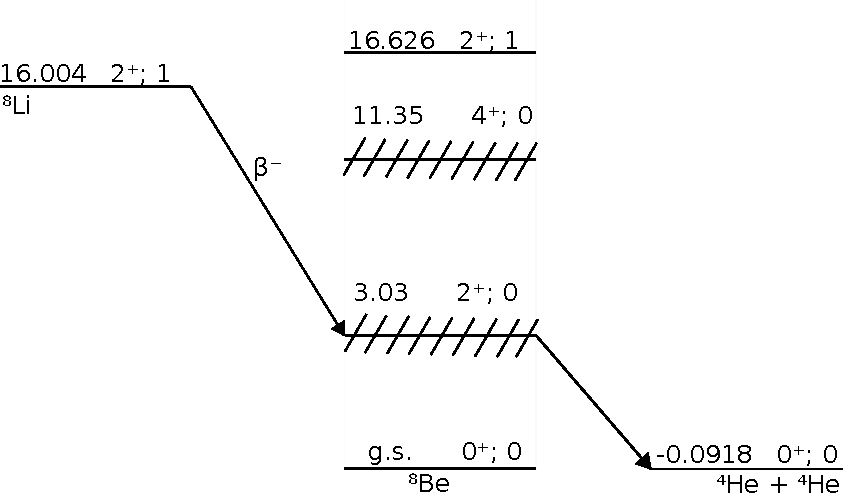
\includegraphics[width=\columnwidth]{../figures/DecayScheme.pdf}
	\caption{The decay scheme of \li, and some notable excitation energies of \ber. Each level is labeld with the energy above the \ber ground state in MeV. Spin parity and isospin is noted as $J^\pi; T$. All information is from \cite{TILLEY2004155}.}
	\label{fig:berStructure}
\end{figure}

	\chapter{Theory}
	\chapter{Experimental Methods}
The main goal of the experiment was to determine the \be-\al\ angular correlation. This was done at the IGISOL facility, at the University of Jyväskylä, where beams of all elements can be produced. The experiment took place in august 2020, due to a delay caused by the ongoing corona pandemic. This chapter will be concerning the experimental setup, a discussion of the detectors and an overview of the software used to extract and analyze the data. 

\section{Detector setup}
The detection setup consists of 6 double sided silicon detectors (DSSD), and 6 single sided silicon detectors (SSD). 
The detectors are $\SI{5}{cm} \times \SI{5}{cm}$ and placed in a cube around the a target in the center, as shown on figure \cref{fig:opstilling}. The setup is designed with measuring the opening angle of the $\beta$ in mind, and therefore the detectors covers 51\% of the solid angle. \\


\section{Experimental setup}
The setup is designed to measure $\beta\alpha$ angular correlations in the $\beta$-delayed particle decay of \isotope[8][]{Li}. When measuring multiple particles, the setup is highly dependent on the coverage of the solid angle. Therefore the setup is designed to have a large solid angle coverage, with high $\alpha$-particle resolution, while still being able to measure $\beta$-particles. \\
This is has been achieved by creating a cube of six double sided silicon detectors (DSSD), all backed by a unsegmented silicon detectors (PAD). To gain the largest solid angle, the detectors where placed as close to one another as possible. A 3D printed case was designed to hold the detectors in place, and achieved a solid angle coverage of 51\% for the DSSD's, which can be seen on \cref{fig:cubepic}. An illustration of the setup, together with the different detectors' thickness can be seen on \cref{fig:opstilling}. 
Even though the setup was designed to hold 12 detectors in total, there where only 11 detectors in the actual experiment. The PAD behind Det1 was defect, and was therefore removed. 

\begin{table}[H]
	\centering
	\begin{tabular}{ll|ll}
		Detector & Thickness {[}$\mu$m{]} & PAD & Thickness{[}$\mu$m{]} \\ \hline
		Det1     & 67                     & n/a & n/a                   \\
		Det2     & 1002                   & P2  & 1036                  \\
		Det3     & 65                     & P3  & 1497                  \\
		Det4     & 60                     & P4  & 1490                  \\
		DetU     & 60                     & PU  & 1498                  \\
		DetD     & 1043                   & PD  & 1038                 
	\end{tabular}
\end{table}

\begin{figure}[h]
	\centering
	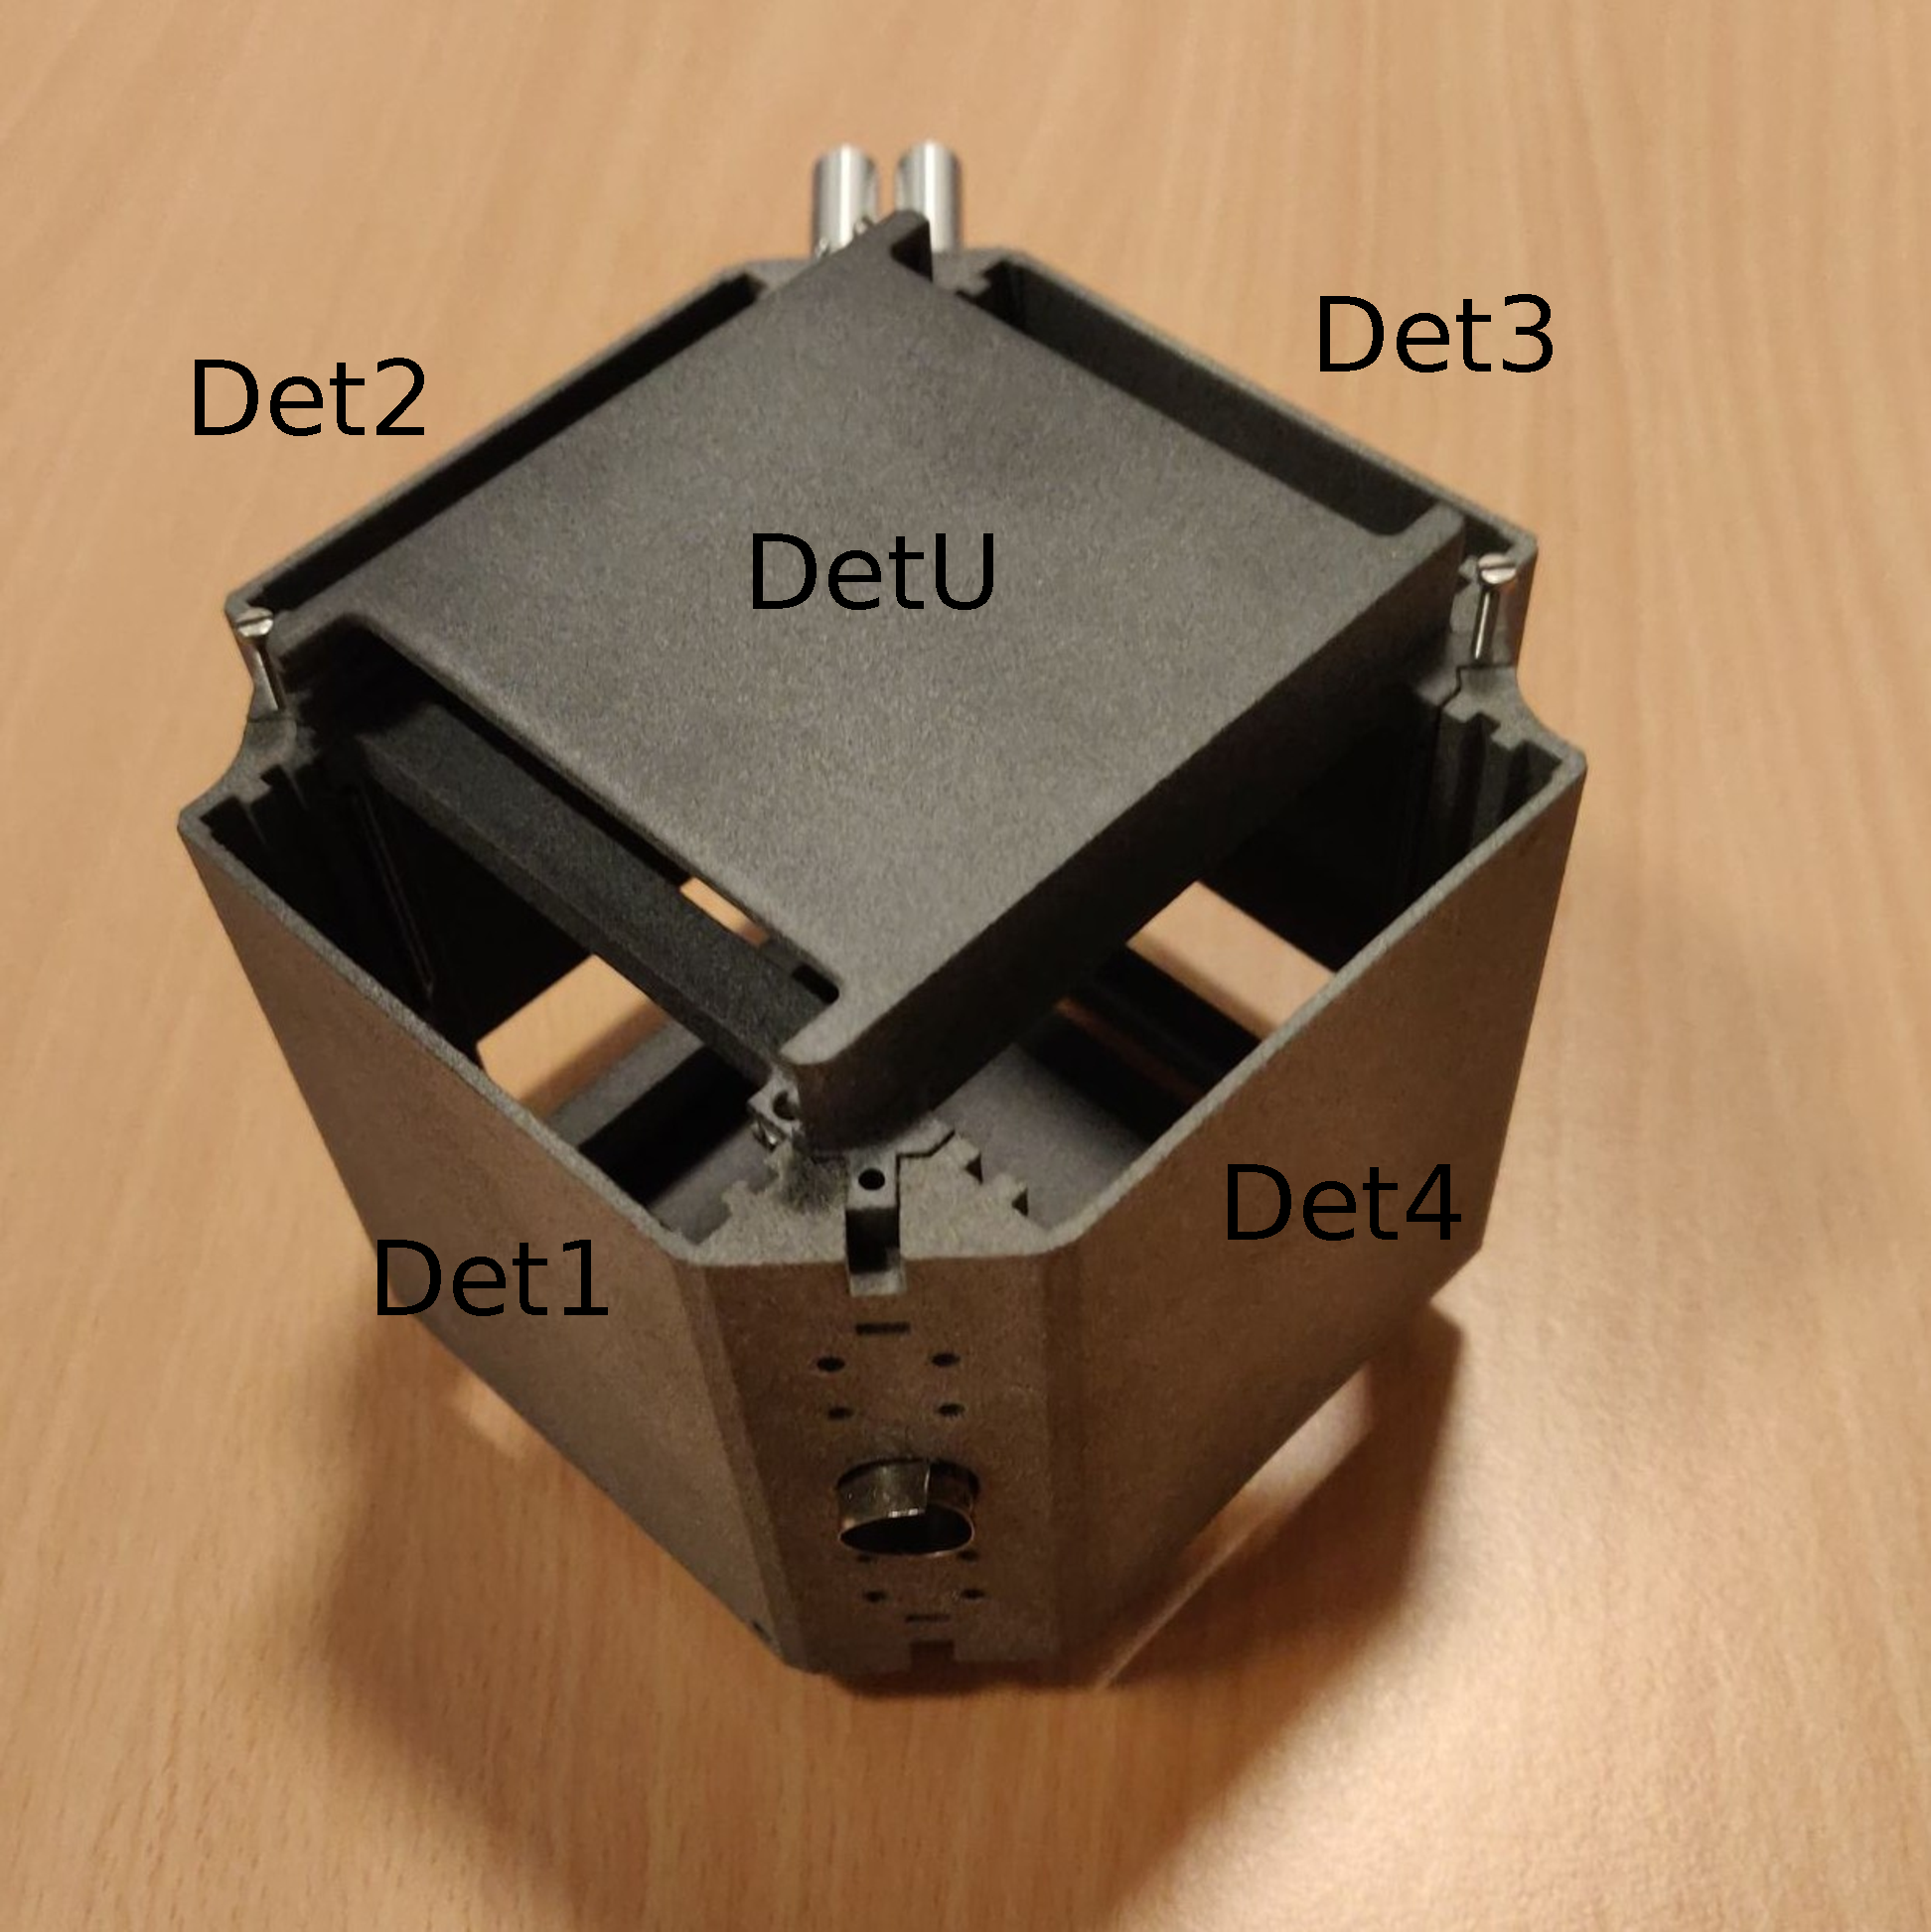
\includegraphics[width=.6\linewidth]{../figures/cubepic.pdf}
	\caption{A picture of the 3D printed cube used to hold all detectors in place. The placement of the detectors have been shown, with exception of DetD, which was at the bottom of the cube. The beam enters the metal ring between Det1 and Det4}
	\label{fig:cubepic}
\end{figure}

\begin{figure}[H]
	\centering
	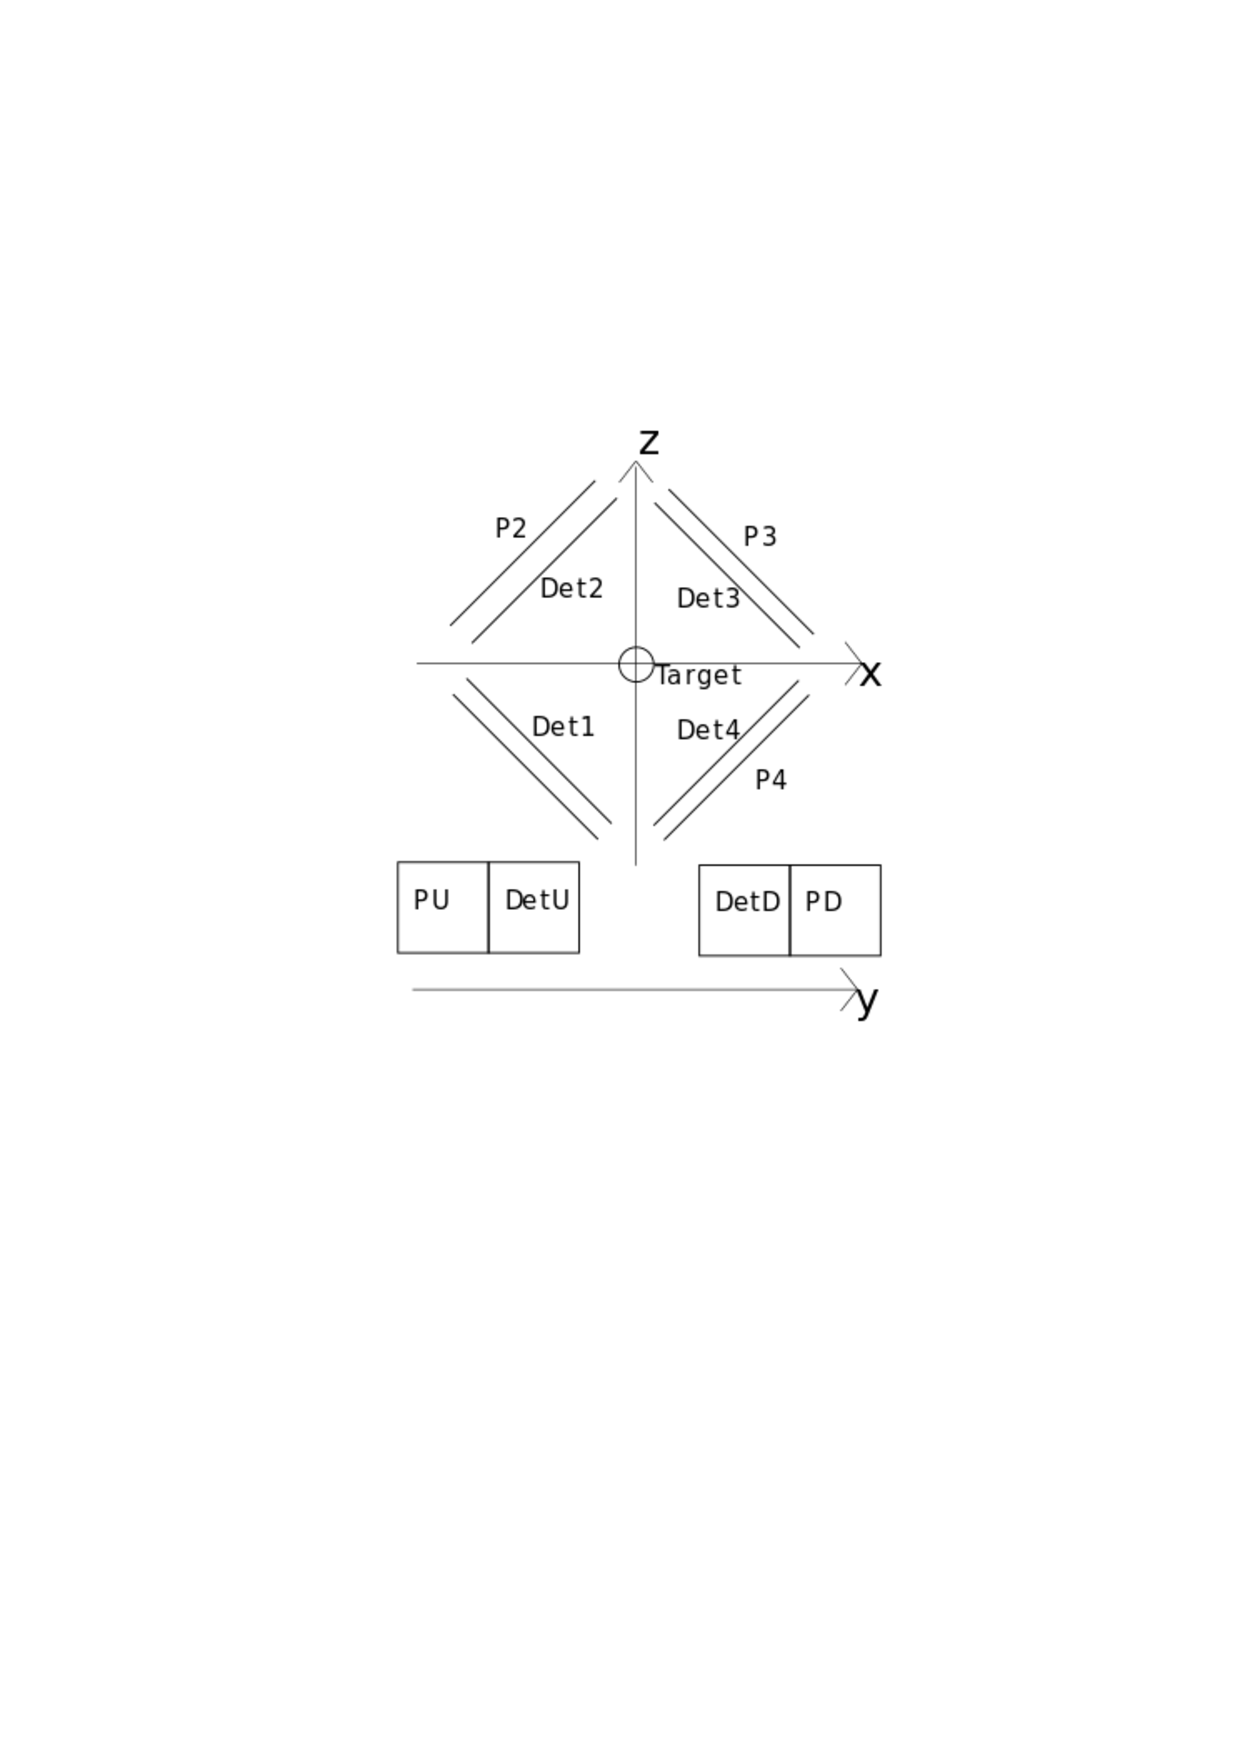
\includegraphics[width=.6\linewidth]{../figures/opstilling_better.pdf}
	\caption{An illustration of the setup. Det1-Det4 are placed around the target, facing the target which is located at the center of the coordinate system. DetU are above the target, and DetD are below the target. Behind each detector is a PAD, with the exception of Det1, who's PAD was defect. The beam is parallel to the z-axis, entering the setup from the negative z-direction.}
	\label{fig:opstilling}
\end{figure}

\section{The detectors}
As mentioned above, there where two types of detectors present in the setup. The first type is the Double sided silicon detector. 
As the name suggests, it consists of two sides, a front layer and a back layer. Each layer consists of 16 strips, that are placed in rows next to each other. The two layers are then arranged so each side are mutually orthogonal, which effectively makes pixels where each strip intersects a strip on the other side. An illustration of the detector can be seen on \cref{fig:W1}.\\
The strips on the front side are p-doped, while the back side are n-doped. When a charged particle hits the detector, it will ionize the atoms in the semi-conductor, and produce a electron-hole pair. The number of electron-hole pairs is proportional to the energy of the charged particle. 
The bias voltage on the detector collects the electrons and holes on opposite sites of the strip, where the charge is collected on aluminum contacts and a signal is measured. Energy is not deposited in these contacts, and therefore they constitute to a so called dead layer. \\
The detectors are square $5\times 5$ \SI{}{cm} and with their $16\times 16$ strips, they have an effective gird of  256 pixels of \SI{9}{mm}. 
4 of the 6 detectors have a thickness of \SI{60}{\mu m} and a dead layer of \SI{100}{nm} dead layer. These detectors are the ones called Det1, Det3, Det4 and DetU in the setup seen on \cref{fig:opstilling}. The other 2 detectors (Det2 and DetD) where both \SI{1000}{\mu m}.
\\
\\
The other type of detector was the PADs. They are different from the DSSD's, in that they do not have sides, and no strips. Therefore they do not contain a grid, the same way the DSSD's do, and will not provide any information as to where a particle has hit. But they are included in the setup to detect excess energy of particles not stopped by the DSSD. This makes them good at detecting \be-particles, as they will not be stopped by a DSSD.

\begin{figure}[h]
	\centering
	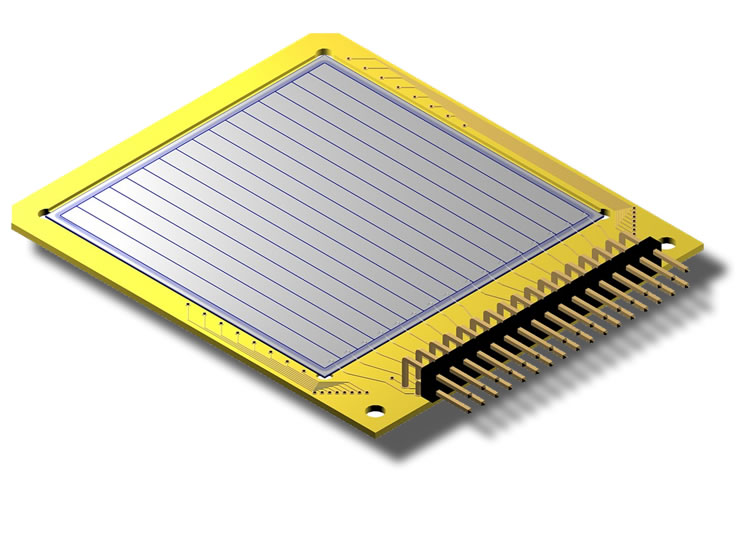
\includegraphics[width=\columnwidth]{../figures/W1.jpg}
	\caption{An illustration of the DSSD type used in this experiment. The detector has 16 p-doped strips, and 16 n-doped strips perpendicular to these. This gives 256 pixels for the detector. Image courtesy of Micron Semiconductor Ltd}
	\label{fig:W1}
\end{figure}

An $\alpha$-particle will deposit all of its energy into the first DSSD it encoutner, and be effectively stopped completely by it, and a a $\beta$-particle will deposit almost no energy in a thin DSSD, and travel through it, ending up depositing some energy in the PAD. \\
Therefore one can roughly distinguish the $\alpha$-particles from the $\beta$-particles, by observing whether a particle has hit the DSSD and the PAD. \\
\\
Since there are also two thick DSSD's in the setup, one can also get some information from a $\beta$-particle from these thicker detectors, as it will deposit more energy in these detectors. 




\section{AUSAlib and ROOT}
ROOT \cite{ROOT} is an object oriented C++ framework that is designed primarily for data analysis in high-energy and nuclear physics. It was created at CERN in 1995, and has since grown and become the dominant analysis software at both CERN and many other nuclear and particle physics laboratories. 
ROOT was designed to handle large amounts of data with high computing efficiency. \\
ROOT makes an intelligent data structure by creating a "Tree" with the class \texttt{TTree}. This tree will then have "branches" which corresponds to some variable of the given detection event, such as the energy of the front strip or identity of the detector. This TTree then allows for reading of an individual branch, while ROOT takes care of the memory management. One can also store a TTree to the disk in the form a .root file. \\

ASUALib \cite{AUSA} is a tool that build on top of ROOT. It was created by the subatomic group at Aarhus University.
Before this tool was created, everyone in the group had to more or less create their own tools to get data from the detectors into a useful data structure. This meant that a lot of time was wasted just trying to access data from experiments. AUSAlib was therefore created, so the basic tasks of data extraction was automated. \\
AUSAlib has a lot of functionalities, but the two main tools that was used to extract data was the \textit{Sorter} and \textit{Calibrator}.

\subsection{Unpacker}
The \texttt{Unpacker} converts raw data from the detectors into a ROOT TTree. This is done by using the unpacking program \texttt{ucesb} \cite{ucesb}. This will setup the branch structure of the data. Some of these branches are \texttt{FT} and \texttt{BT}, which is a vector of the  \texttt{TDC} (time) values for each event, for the front and backside of the detector. They are vectors because they contain information for each particle hits in a given time slot, for which there can be multiple. 
There are also the branches \texttt{FE} and \texttt{BE}, which is the \texttt{ADC} (energy) associated with the events. 

\subsection{Calibrator}
Since the detectors work, by measuring an electrical charge that comes from the charged particle, the detectors needs to translate a specific charge to energy deposited. \\
To do that, we use the \texttt{Calibrator}-tool, which is designed to convert a channel number into an actual energy. Assuming that the channel numbers are linearly related to the energies, a known radioactive source can be measured, and the expected spectrum can be compared to the measured. This is done for each strip in each detector.
\\
\\
The \texttt{Calibrator} starts by running a peak-finding algorithm over some calibration data, to roughly identify the locations of the peaks, followed by a multi-Gaussian fit to find the most precise peak location. 
The positions of the peaks can then be compared to the expected energies, giving an associated energy to a given channel. \\
\\
As mentioned earlier, all of the detectors have a small aluminum dead layer. All particles that pass through this layer will loses some amount of energy depending on the stopping power of the material and the effective thickness of the dead layer $\Delta x_{eff}$, which furthermore depends on the angle of incidence, $\theta$. 
The relationship between the effective thickness and the actual thickness is described as $\Delta x_{eff} = \Delta x/ \cos(\theta)$. This gives the measured energy as 
\begin{equation*}
E' = E - \dfrac{dE}{dx} \dfrac{\Delta x}{\cos(\theta)},
\end{equation*}
where $E$ is the original energy of the particle, $dE/dx$ is the stopping power of the material and $\Delta x$ is the thickness of the dead layer. The stopping power is calculated from SRIM \cite{ZIEGLER20101818} \\
\\
These calculations are all handled by the \texttt{Calibrator}. 
As input it takes an unpacked measurement of a source, a file specifying the locations of the expected peaks and a file specifying the spacial locations of the detectors. 
From this it calculates the energy loss, and creates a linear relationship between channel numbers and energies. This is then written to the disk as a seperate calibration file, which can be parsed to other modules.\\
It is important to note that the Calibrator does not modify any data. Therefore the energy loss is unaccounted for. Instead it corrects the expected energy spectrum, which means that the resulting calibration is still valid. The energy loss correction is therefore still needed in the analysis, as the effect is unaccounted for in measurements. 


\subsection{Sorter}
The sorter is used after a successful calibration. It generates a ROOT file based on the unpacked data, and applies the calibration. 
It is also responsible for matching and combining events from the front-side to the back-side of the detector. If there where one hit in the front side and one in the back, the mathcing is fairly trivial. If there however where multiple hits in both front and back, the \texttt{Sorter} will run a matching algorithm, which pairs the hits with the lowest energy differences. \\
\\
When the events have been matched, the hits on the individual sides of each detector are merged into a single event. 
Therefore each event can now be considered a multiple of particle hits. This makes it possible to to associate physical properties with each particle, such as direction and energy. 
There has still not been done any filtering of the data, which is what we will discuss in  \cref{cha:dataReduction}.



	\chapter{Data Reduction}
\label{cha:dataReduction}
\section{Calibration}
To actually calibrate the detectors, we use an $\alpha$-source with a known spectrum. The source is placed in the target position, and each detector is in turn placed in front of the source. 
The radioactive source used to calibrate this setup contained \isotope[148][]{Gd}, \isotope[239][]{Pu} and \isotope[244][]{Cm}. Each isotope has a prominent main peak, and several sub peaks. The proprieties of which is listed in  \cref{tab:cali}.
\begin{table}[H]
	\centering
	\begin{tabular}{ll}
		Isotope & $E_\alpha \ [keV]$  \\ \hline
		\isotope[148][]{Gd}		& 3182.690         \\
		\isotope[239][]{Pu}		& 5105.5           \\
								& 5144.3           \\
								& 5156.59          \\
		\isotope[244][]{Cm}		& 5762.64          \\
								& 5804.96          \\ 
	\end{tabular}
	\caption{Decay energies for each isotope used in the calibration.}
	\label{tab:cali}
\end{table}
A typical single strip spectrum is shown on \cref{fig:singleStripExample}, where the calibrator has given an estimate of where the peaks are, illustrated by the red triangles. \cref{fig:peakExample} shows a closer look at the \isotope[244][]{Cm} peak, where the red line shows the \texttt{Calibrator}-fit over both the main peak and the sub peak. \\

\begin{figure}[H]
	\begin{subfigure}{\linewidth}
		\centering
		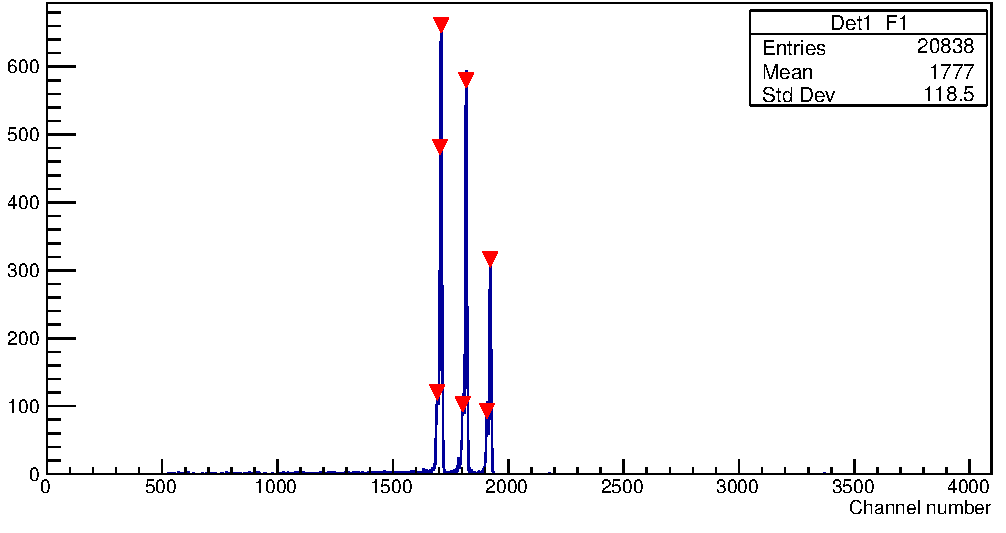
\includegraphics[width=.9\linewidth]{../figures/cali/det1f1-cropped.pdf}
		\caption{A spectrum of the calibration source, with channel number along the x-axis. The red triangles indicate the positions the \texttt{Calibrator} has guessed as the peaks.}
		\label{fig:singleStripExample}
	\end{subfigure}
	\begin{subfigure}{\textwidth}
		\centering
		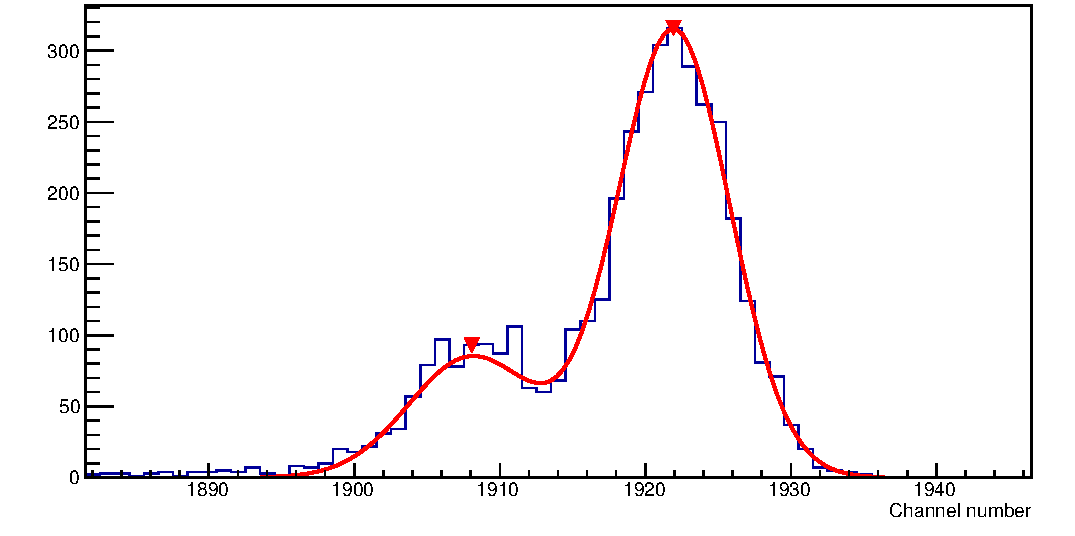
\includegraphics[width=.9\linewidth]{../figures/cali/det1f1PeakMostLeft-cropped}
		\caption{A closer look at the \isotope[244][]{Cm} peak on the above figure. The red line is a fit performed by the \texttt{Calibrator}, and the red triangles indicate the guessed peaks. }
		\label{fig:peakExample}
	\end{subfigure}
	\caption{Calibrations of detector 1}
	\label{fig:CaliExamples}
\end{figure}


\section{Identifying the particles}
After utilizing the AUSAlib tools, the data is ready to be analyzed. Even though the theory dictates that a decay will consist of two \al-particles and one \be-particles, it is not realistic to just assume that each detected event will consist only of this configuration of particles. \\
Therefore we need some cut on what events we will allow through to the analysis. Specifically we are going to impose 3 cuts on the data, a angular cut, a momentum cut and a multiplicity cut.



\subsection{Identifying a hit}
After a hit has been detected, and all the relevant information has been extracted from the hit, we can start to analyze what type of particle has hit the detector. 

A important distinction between an \al-particle and a \be-particle is the different interactions with a detector. An \al-particle will be completely stopped by a standard \SI{60}{\mu m} detector, while a \be-particle will pass through it, depositing only a small amount of energy. \\
This is the reason for the PAD's behind each DSSD. The idea is that only a \be-particle will be detected in the PAD's, so if a hit has some energy in a DSSD \textit{and} the corresponding PAD, it will be classified as a \be-particle.\\
\\
This approach however does not work as well as intended. Often what happens is that the thin DSSD will not pick up any energy deposited, and the hit will therefore not be counted. 
But not all of the detectors are \SI{60}{\mu m}. We have two detectors that are around \SI{1000}{\mu m} thick. These detectors are much better at picking up a signal from a \be-particle, so one of the criteria for being a \be-particle in this setup is to have hit either Det2 or DetD.\\

These two criteria are however not enough to uniquely determine that a hit was a \be-particle. We still have to consider the events where a detector has multiple hits. Since a PAD gives no usable information regarding where a particle has hit, we cannot say which particle was a \be-particle and which where an \al-particle. 

Therefore if the \be-particle criteria are true, we mark the particle as a \textit{possible} \be. But since it might as well have been a \al-particle, we also mark it as such.\\
Every hit that does not uphold to the \be-particle criteria are of course marked only as a possible \al-particle.
\\
%When a particle is marked as a \al-particle, we also perform an energy correction, \textcolor{red}{MAYBE ENERGY CORRECTION HERE??}
%
When all the particles have been identified, we impose the first cut to the data. A multiplicity cut that says we need at least two \al-particles. If there are less, we discard the event. 
\\
When we at least have two distinct particles that can be \al-particles, we look at their mutual difference in momentum. The particle pair with the least difference in momentum will be chosen as the only \al-particles that can be present in an event. Then we have assured that every other particle we see in the event, is possible \be-particle candidates. 
\\
When each particle has been identified or discarded, all remaining particle-specific information is stored to the given particle for easy analysis henceforth.

\section{Angular cut}
When \isotope[8][]Be decays, and produces the two \al-particles, it will do so under conservation of momentum. The decay in any direction, but the angle $\theta$ between them will be close to  $180\degree$. Therefore the first cut that we give to the data, is that two of the particles that are \al\ candidates, must have a mutual angle of close to $180\degree$.\\


On \cref{fig:cosAll} a plot of all the the mutual angles are shown. A quick glance will give that most particles will have mutual angle of close to $180\degree$. 

\begin{figure}[h]
	\centering
	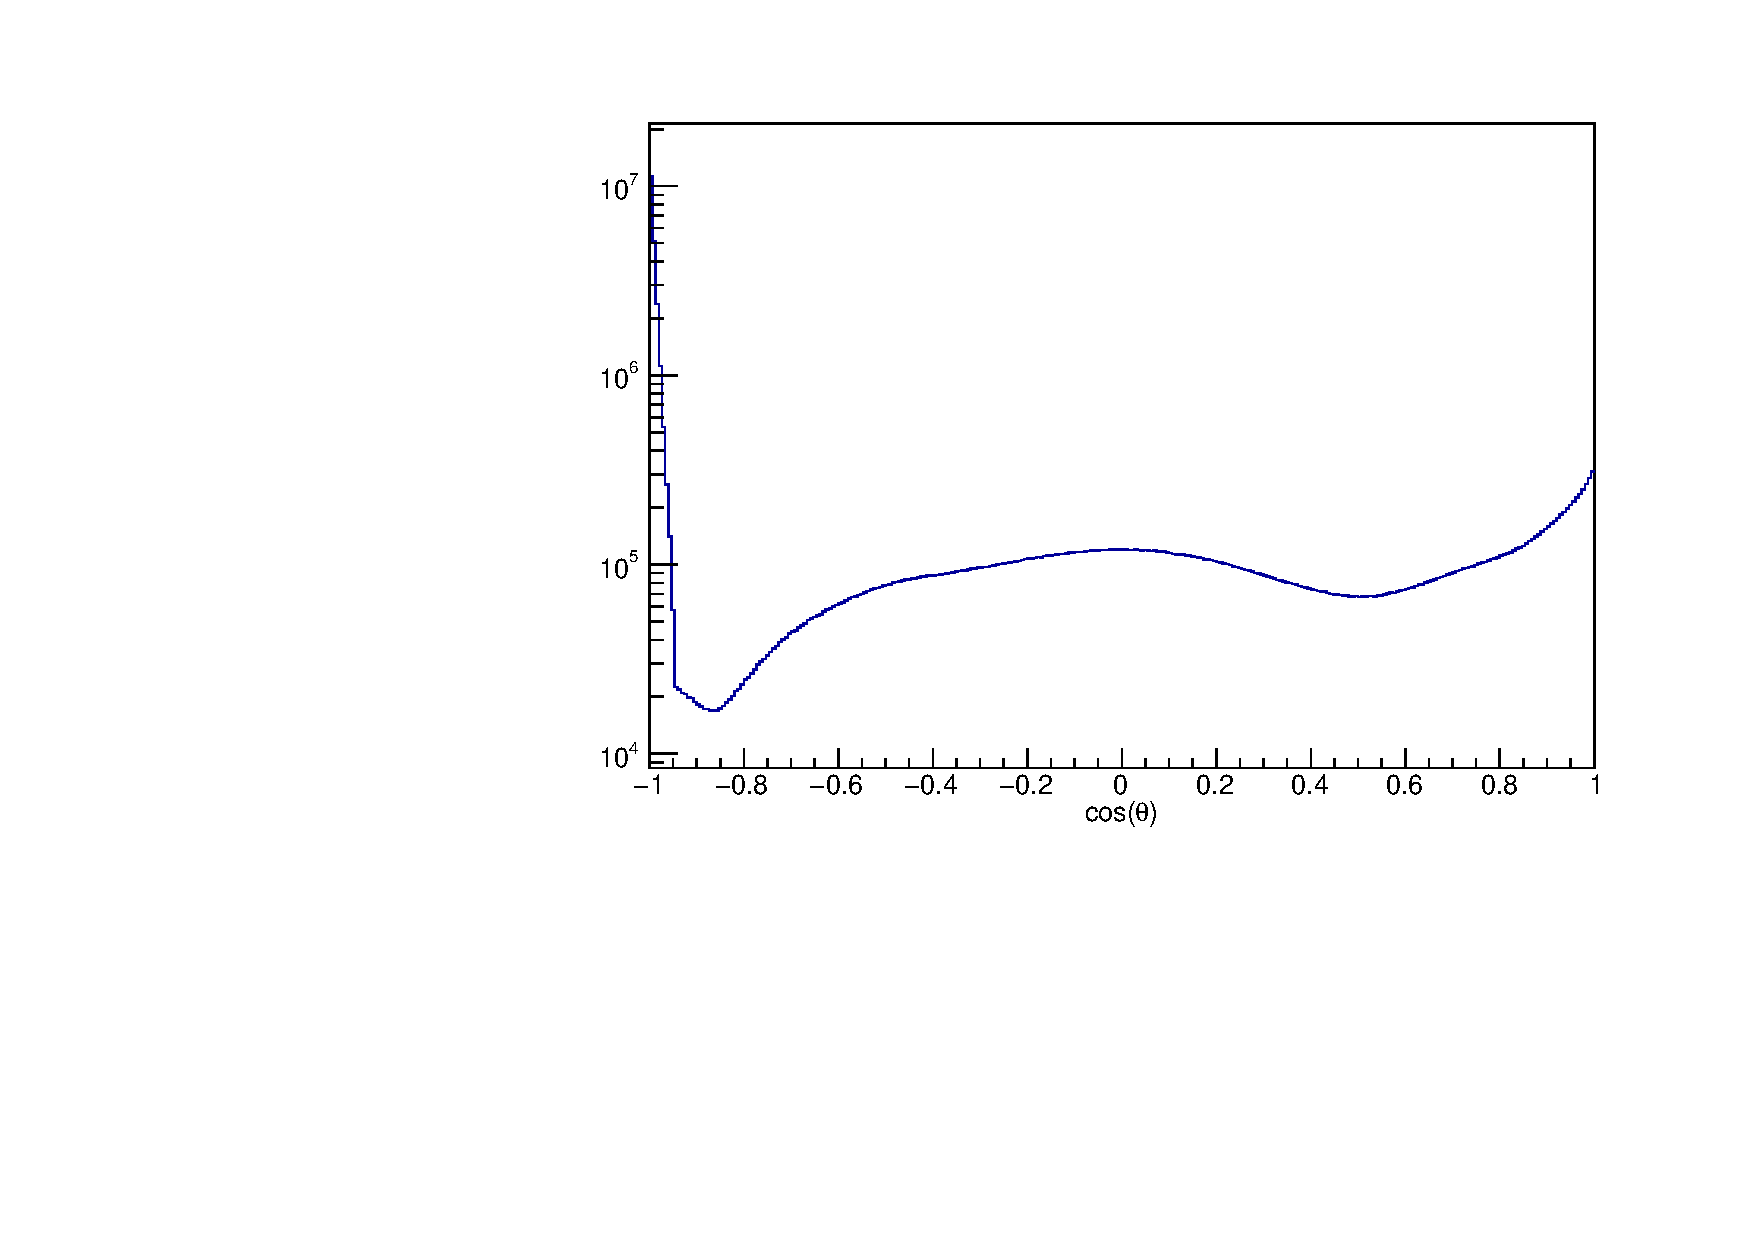
\includegraphics[width=\linewidth]{../figures/cosang.pdf}
	\caption{A histogram of all the mutual angles between all particles.}
	\label{fig:cosAll}
\end{figure}

By looking at this, we see that most of the angles will lie close to $180\degree$, and now we must decide exactly where to do the cutoff. 
By taking a sharp cutoff at $\cos(\theta) \geq -0.99$, we will exclude a great deal of good measurements, on the other hand, a too soft cut will not accomplish anything, as too many "wrong" particles will let through the check. By trying different cuts, we have found that $\cos(\theta) \geq -0.95$ is a good cutoff, and this corresponds to 161\degree. 



\section{Momentum cut}
The second cut we perform on the data is a \textit{total} momentum cut. On \cref{fig:totalMomentum} the total momentum for the two identified \al-particles are shown. 
A prominent peak lies around \SI{13.000}{keV/c}, and ends around \SI{40.000 }{keV/c}. 
We impose a cut of maximum \SI{40}{MeV/c}, as this will include the large amount of pairs lying in the peak, which must be \al-\al pairs. A \al-particle with energy \SI{1500}{keV} will have a momentum of \SI{105}{MeV/c}, and a free electron of \SI{3000}{keV} will have a momentum of \SI{1.7}{MeV/c}. 
The majority of particles lies around these energies, and no matter where the \be-particle will hit, the total momentum is still much larger than the \SI{40}{MeV/c} cutoff. 
\begin{figure}[h]
	\centering
	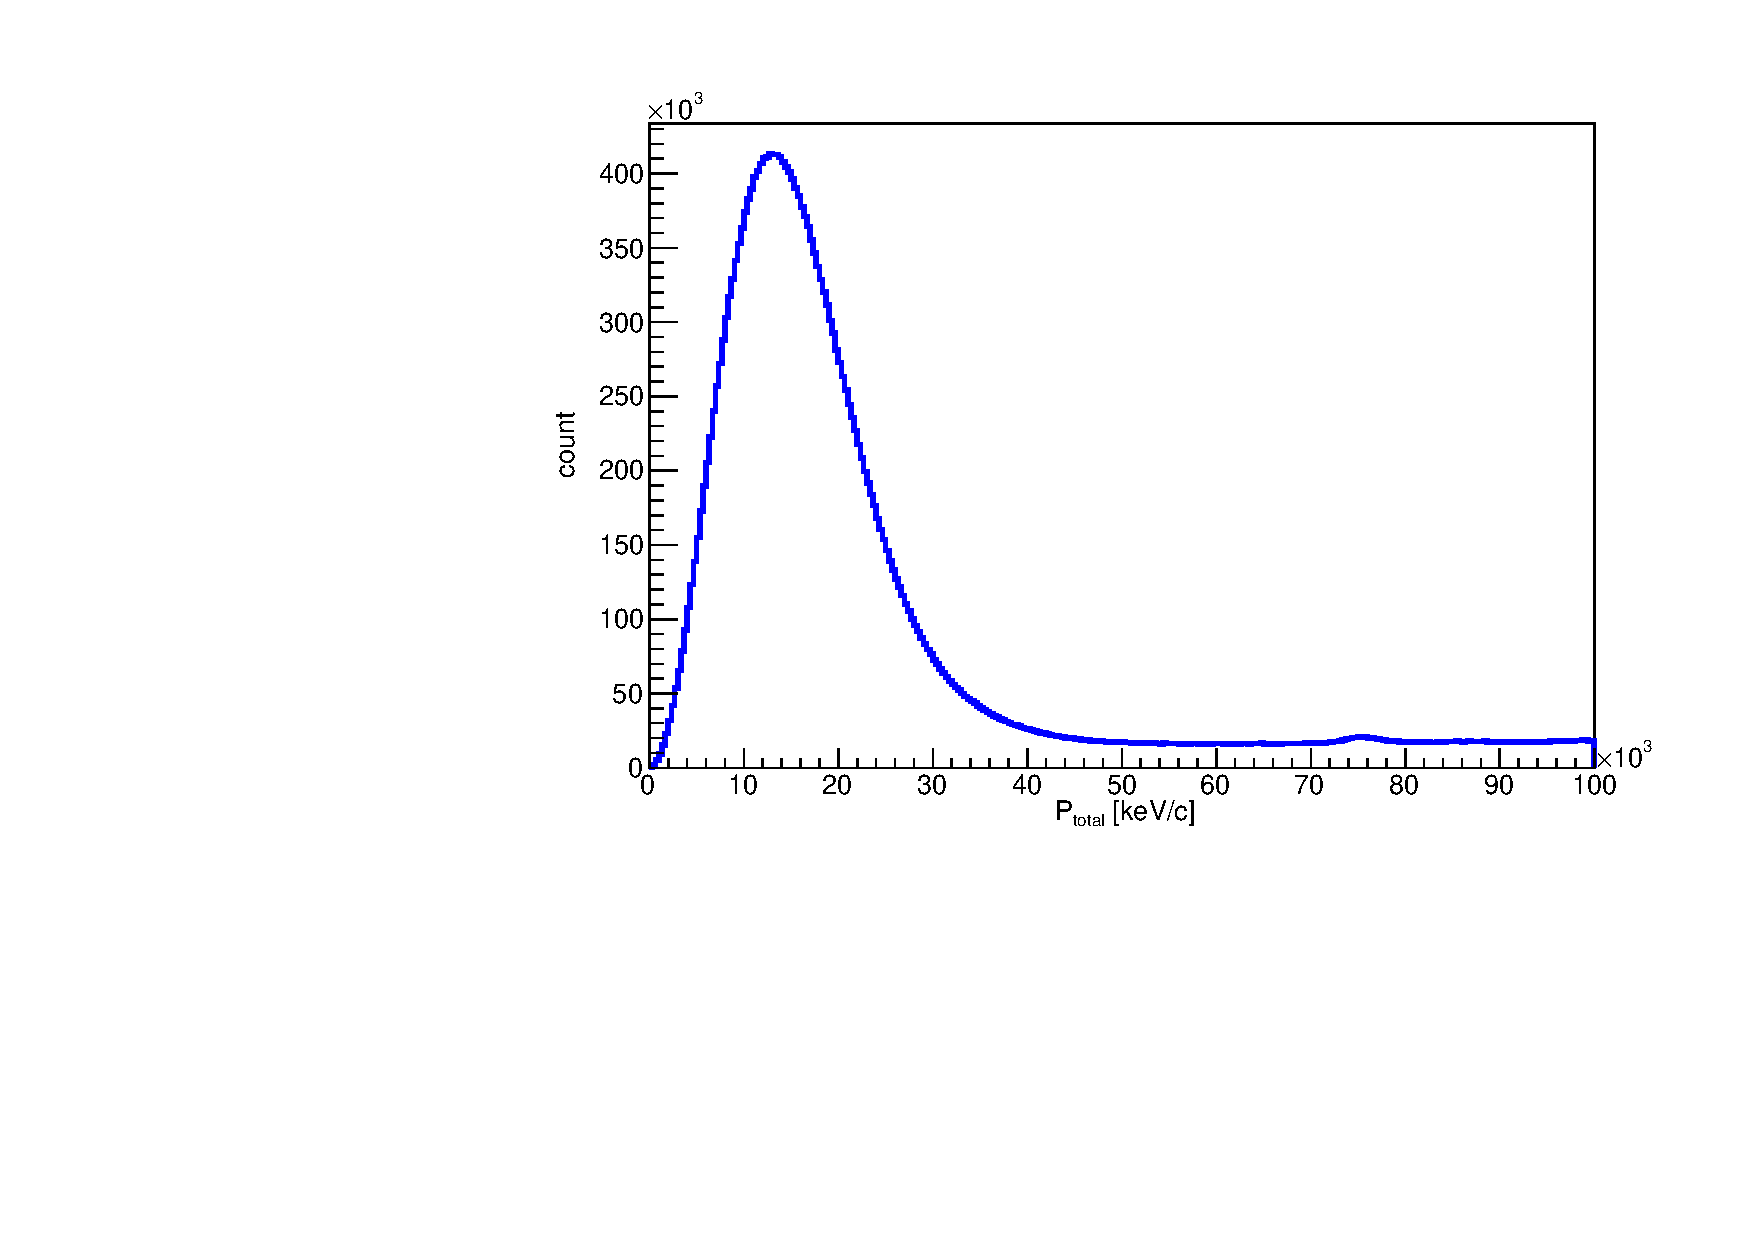
\includegraphics[width=\linewidth]{../figures/ptotNoCut.pdf}
	\caption{The total momentum of the two \al-particles.}
	\label{fig:totalMomentum}
\end{figure}

\section{Multiplicity cut}
The last cut that we want to impose on the data, is a multiplicity cut. This cut is just to ensure that we have the amount of particles that we expect. 
Therefore a hard criteria is that there must be at least two distinctly identified \al-particles. \\

With regards to the \be-particles, we are more loose. Here we say that there must at least be one, but more can occur. This is quite rare, but the we still take that event into account, as the \be-particles should have an isotropic distribution, and therefore should not in any case be affected by the other \al-particles. On \cref{fig:mulBeta} we see the multiplicity of \be-particles, and in most of the events, we have not detected any \be-particles, and when we do, there is a even fewer events with more than one beta. So most of the time, we are in the expected case with two \al-particle and one \be-particle. \note{add that beta spreads around in the setup}

\begin{figure}[h]
	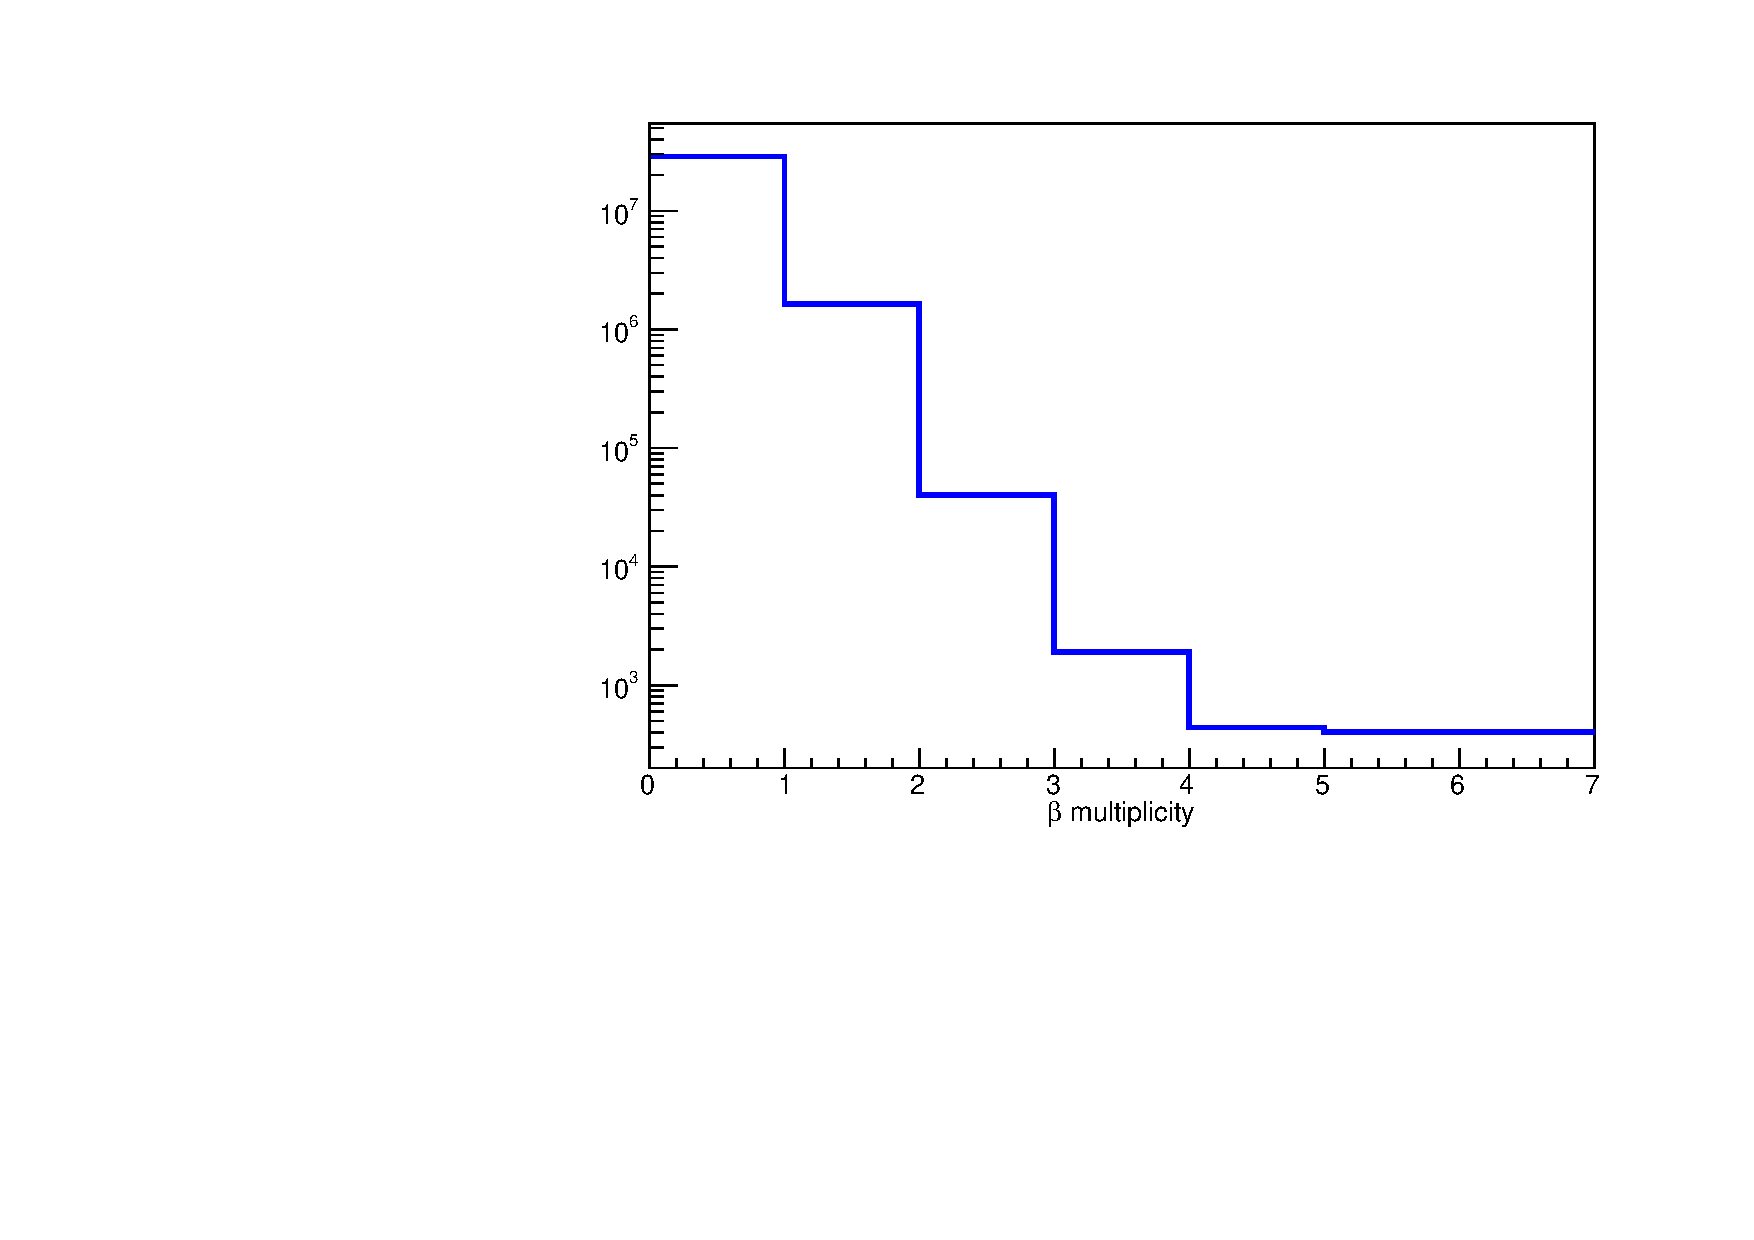
\includegraphics[width=\linewidth]{../figures/betaMul.pdf}
	\caption{The multiplicity of the \be-particles.}
	\label{fig:mulBeta}
\end{figure}
	\chapter{Conclusion}
With coincidence measurements of \be-delayed \al-\al breakup of \li, we have successfully measured the excitation spectrum of \ber. This spectrum has been compared to previous more precise measurements, and a nice consensus between the shape of the two measurements are shown. 
\\
\\
The primary goal of the experiment was to measure the \be-\al\ angular correlations in the decay of \li, since it is previously shown that this would be isotropic. 
Two decays was measured using this setup, \li and \isotope[12]{B}, which involves a triple \al-decay, and a \be-decay. The setup was designed to measure \al-particles position and energy with high resolution, as well as detecting \be-particles position to equal resolution. 
\\
By comparing the excitation spectra of \ber, to previous measurements, we have shown that the setup has a satisfied energy resolution for \al-particles. This has been further enhanced as it is shown that a good coincidence sorting will give a more precise \al\ energy resolution.\\
When it comes to the \be-\al\ angular correlation, we have shown that there are some inconsistencies in the setup, that causes the angular analysis to more complex than first assumed. There is a good indication of the beam not hitting the exact center of the target, but there is also evidence of some detectors not being placed in a perfect cube around the target. \\
The target holder also casts a shadow on two of the detectors, which can further skew the measured angles away from the expected.

	
\end{document}